\documentclass[tikz,border=12pt]{standalone}
\usepackage{graphicx}
\usepackage{amsmath,amssymb}
\usepackage{tikz}
\usetikzlibrary{arrows.meta,positioning,fit,calc,backgrounds}
\tikzset{
  box/.style={
    draw,
    very thick,
    rectangle,
    align=center,
    inner sep=8pt,
    minimum height=1.25cm,
    minimum width=3.1cm,
    font=\small,
  },
  wide/.style={box, minimum width=3.6cm},
  arr/.style={-{Stealth[length=2.6mm, width=2mm]}, thick},
  barr/.style={
    {Stealth[length=2.4mm, width=1.8mm]}-{Stealth[length=2.4mm, width=1.8mm]},
    thick,
  },
  lbl/.style={font=\scriptsize, inner sep=2pt, fill=white},
  group/.style={draw, dashed, inner sep=12pt},
}

\begin{document}
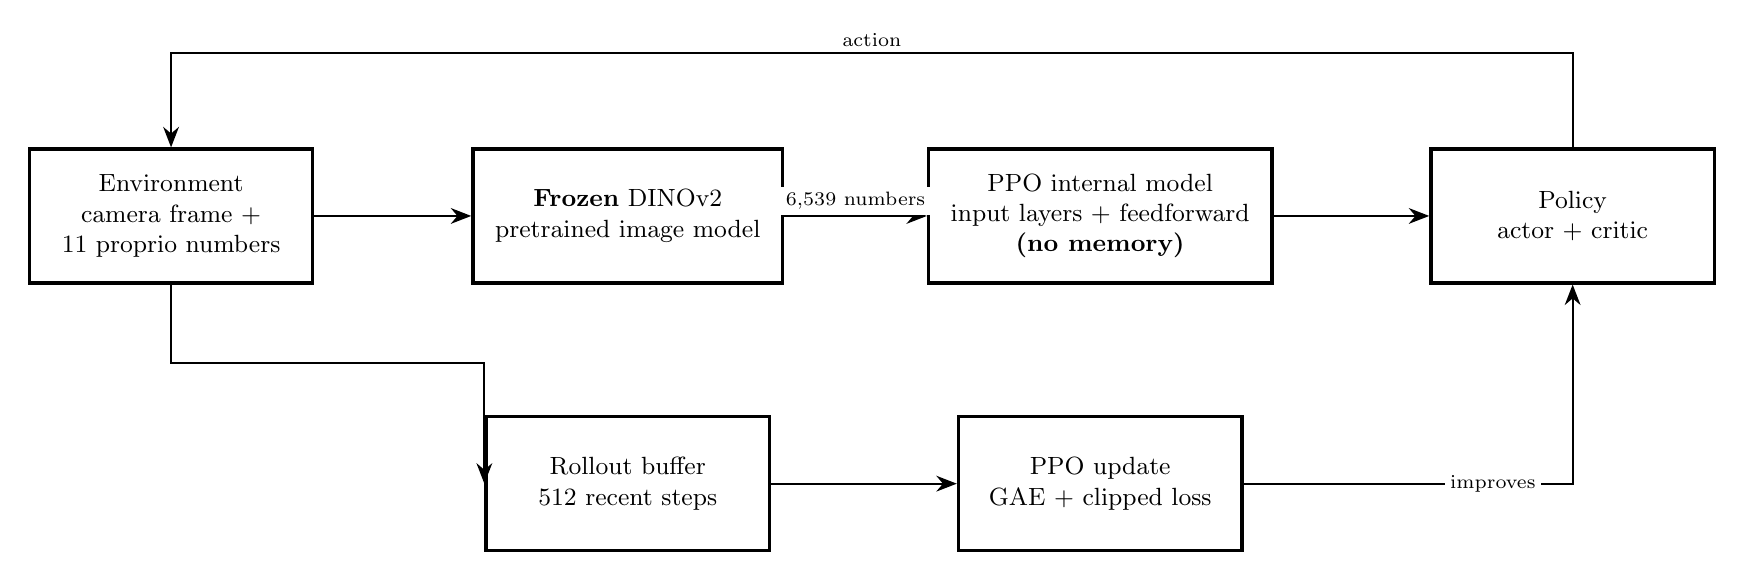
\begin{tikzpicture}
  \tikzset{box/.append style={minimum width=3.6cm, minimum height=1.7cm, font=\small}}
  % acting loop
  \node[box] (env) at (0,0) {Environment\\camera frame +\\11 proprio numbers};
  \node[box] (enc) at (5.8,0) {\textbf{Frozen} DINOv2\\pretrained image model};
  \node[box] (mid) at (11.8,0) {PPO internal model\\input layers + feedforward\\\textbf{(no memory)}};
  \node[box] (pol) at (17.8,0) {Policy\\actor + critic};
  \draw[arr] (env) -- (enc);
  \draw[arr] (enc) -- node[lbl, above] {6{,}539 numbers} (mid);
  \draw[arr] (mid) -- (pol);
  \draw[arr] (pol.north) -- ++(0,1.2) -| node[lbl, above, pos=0.25] {action} (env.north);

  % learning
  \node[box] (buf) at (5.8,-3.4) {Rollout buffer\\512 recent steps};
  \node[box] (upd) at (11.8,-3.4) {PPO update\\GAE + clipped loss};
  \draw[arr] (env.south) -- ++(0,-1.0) -| (buf.west |- buf.west);
  \draw[arr] (buf) -- (upd);
  \draw[arr] (upd.east) -- ++(0.9,0) -| node[lbl, right, pos=0.25] {improves} (pol.south);
\end{tikzpicture}
\end{document}
